\documentclass{article}
\usepackage{mathbbol}
\usepackage{graphicx}

\graphicspath{ {./images/} }
\renewcommand{\arraystretch}{2.5}
\newcommand{\definition}[1]{\paragraph*{\underline{Definition}: #1}}
\newcommand{\property}[1]{\paragraph*{\underline{Property}: #1}}
\newcommand{\theorem}[1]{\paragraph*{\underline{Theorem}: #1}}

\title{Sequence and recurrence}
\author{Flydexo}

\begin{document}
\maketitle
\tableofcontents
\section{Reasoning by recurrence}
\theorem{}
$P(n)$ a property, we suppose that:
\begin{itemize}
    \item $P(0)$ is true
    \item if $P(n)$ is true so $P(n+1)$ is true
\end{itemize}
So for every $n$, $P(n)$ is true
\theorem{Reasoning by recurrence from a certain rank}
$n_0 \in \mathbb{N}$, $n \ge n_0$, we suppose that:
\begin{itemize}
    \item $P(n_0)$ is true
    \item if $n \ge n_0$, $P(n)$ is true so $P(n+1)$ is true
\end{itemize}
So for every $n \ge n_0$, $P(n)$ is true
\paragraph{\underline{Steps to demonstrate by recurrence with $n \ge n_0$}}
\begin{enumerate}
    \item Initialization, verification of the truth of the property for $n=n_0$
    \item Heredity, we suppose $P(n)$ is true, demonstrate that $P(n+1)$ is true
    \item Conclusion, we conclude that $P(n)$ is true for all $n \ge n_0$
\end{enumerate}
\property{Inequality of Bernoulli}
$$a \in \mathbb{R}^*, n \in \mathbb{N}, (1+a)^n \ge 1+na$$
\section{Limit of a sequence}
\definition{Sequence diverging to infinity}
$(u_n)$ tends to $+\infty$ when $n$ tends to $+\infty$, if for every real:
$A>0$ the interval $]A;+\infty[$ includes all the terms of the sequence from a certain rank. We say that $(u_n)$ diverges $$\lim_{n \to +\infty} u_n = +\infty$$

$(u_n)$ tends to $-\infty$ when $n$ tends to $+\infty$, if for every real $A > 0$ the interval $]-\infty;-A[$ includes all the terms of the sequence from a certain rank. $(u_n)$ diverges. $$\lim_{n \to +\infty} u_n = -\infty$$

\definition{Sequence converging a real number}
$(u_n)$ tends to the real $l$ when $n$ tends to $+\infty$ if all the opened interval including $l$ includes all the terms of the sequence from a certain rank. $(u_n)$ converges $$\lim_{n \to +\infty} u_n = l$$

\theorem{Unicity of the limit}
If a limit exists, it is unique.

\section{Property of limits}
\property{Limits of the reference sequences}
$\sqrt{n}, n$ and $n^k$ where $k \in \mathbb{R}^*$ have 
$$\lim_{n \to +\infty} = +\infty$$
$\frac{1}{\sqrt{n}}, \frac{1}{n}, \frac{1}{n^k}$ have $$\lim_{n \to +\infty} = 0$$
\property{Sum and products of limits}
\begin{center}
    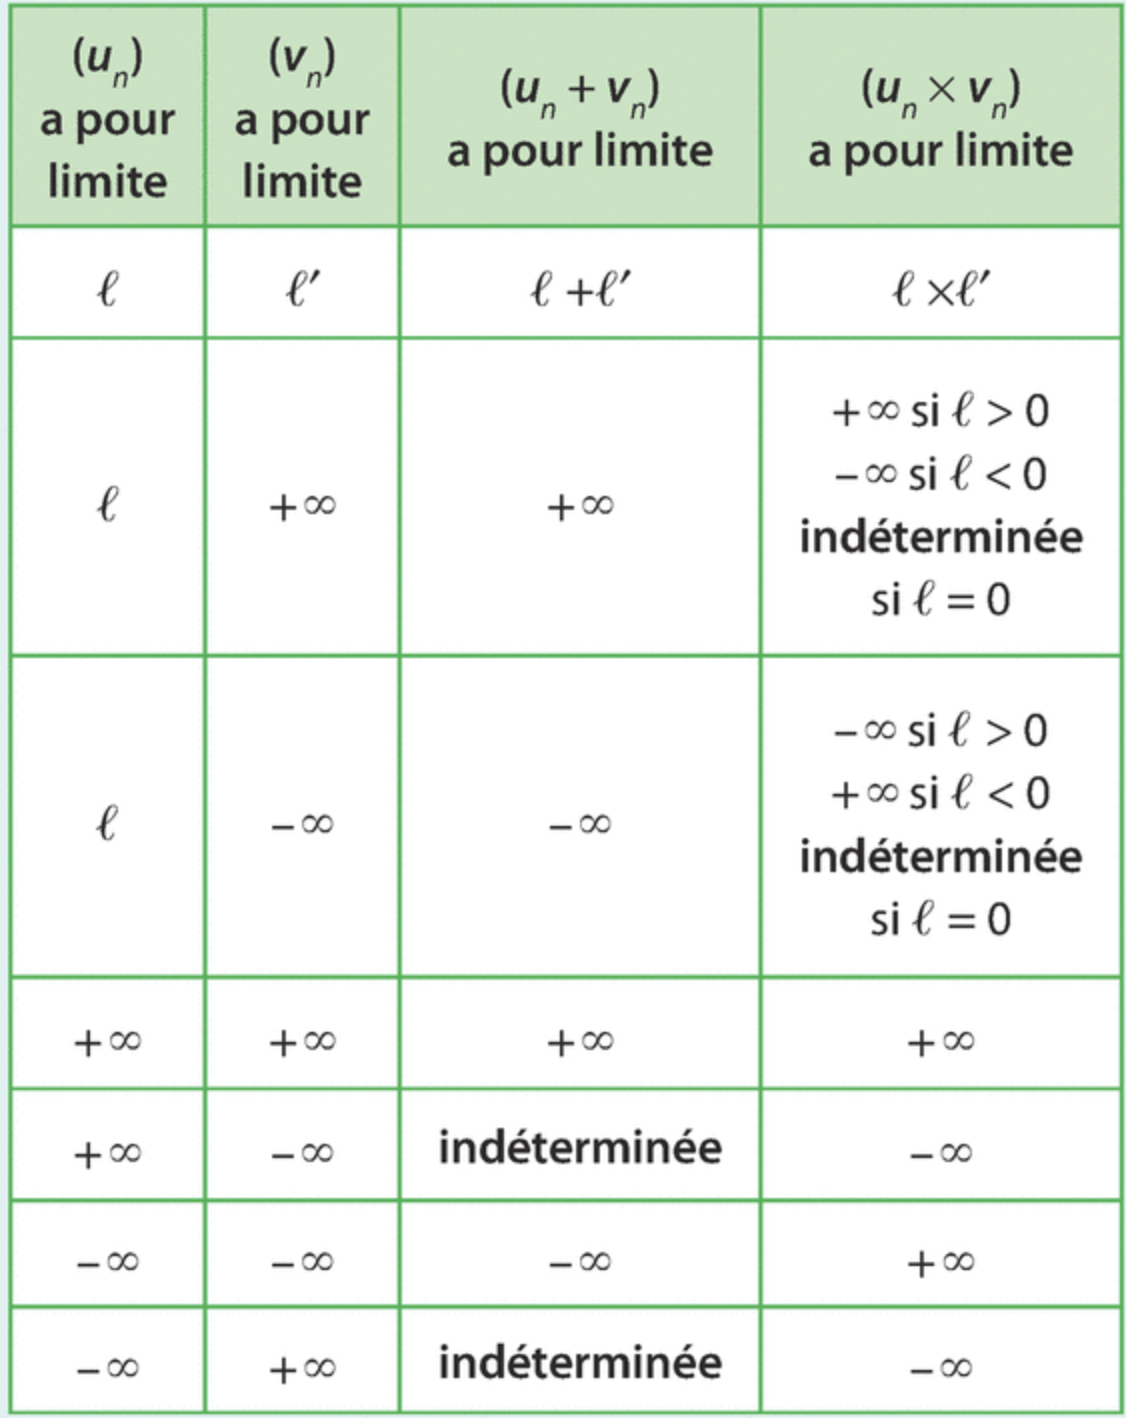
\includegraphics[scale=0.35]{sum_product_table.png}
\end{center}
\property{Quotient of limits}
\begin{center}
    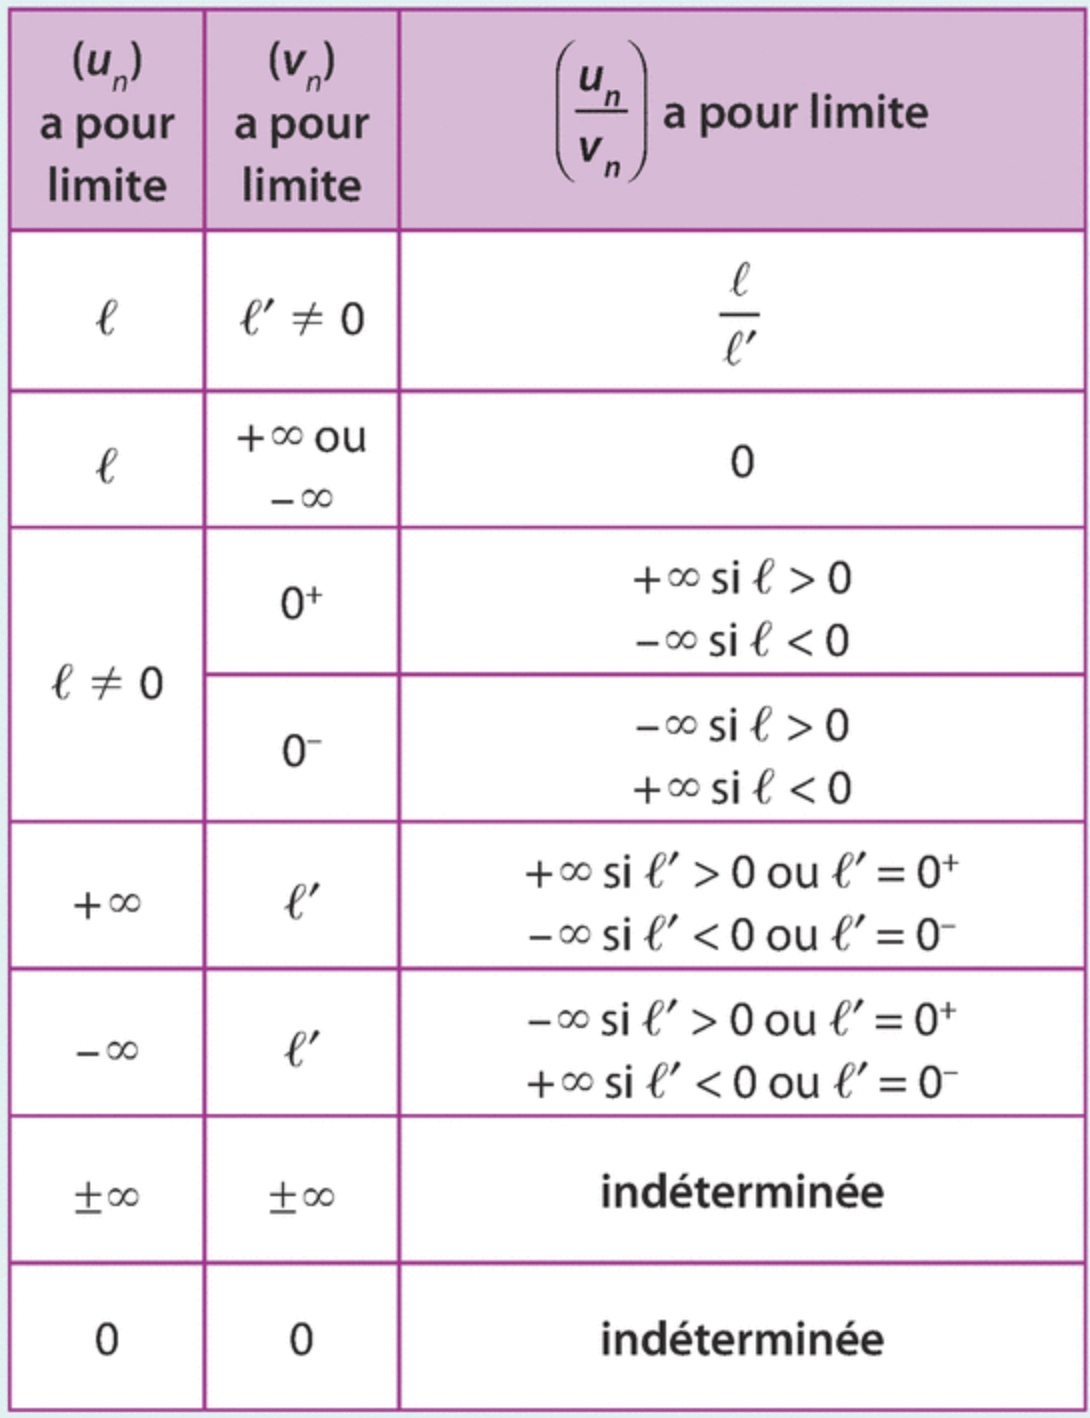
\includegraphics[scale=0.35]{quotient_table.png}
\end{center}
\section{Limit and comparison}
\theorem{Theorem of comparison}
$(u_n)$ and $(v_n)$, $n \ge n_0$, $u_n \le v_n$
\begin{itemize}
    \item If $\lim_{n \to +\infty} u_n = +\infty$ then $\lim_{n \to +\infty} v_n = +\infty$
    \item If $\lim_{n \to +\infty} v_n = -\infty$ then $\lim_{n \to +\infty} u_n = -\infty$
\end{itemize}
\theorem{Theorem of gendarmes}
$(u_n), (v_n), (w_n), l$ a real. 

We suppose that:
\begin{itemize}
    \item $n_0$ exists, such as, $n \ge n_0, v_n \le u_n \le w_n$
    \item $\lim_{n \to +\infty} v_n = \lim_{n \to +\infty} w_n = l$
\end{itemize}
So the sequence $(u_n)$ converges and $\lim_{n \to +\infty} u_n = l$
\property{Inequalities and limits}
Let $(u_n)$ and $(v_n)$ two sequences converging. We suppose $n_0$, such as $n \ge n_0$, $u_n \le v_n$. So $\lim_{n \to +\infty} u_n \le \lim_{n \to +\infty} v_n$ 
\section{Geometrical sequences and monotone sequences}
\property{Limit of a geometrical sequence}
Let $q$ a real.
\begin{itemize}
    \item If $q > 1$, so $\lim_{n \to +\infty} q^n = +\infty$
    \item If $q = 1$, so $\lim_{n \to +\infty} q^n = 1$
    \item If $-1 < q < 1$, so $\lim_{n \to +\infty} q^n = 0$
    \item If $q \le -1$, so the sequence $(q^n)$ has no limit
\end{itemize}
\definition{Increased, understated, bounded sequence}
Let $(u_n)$ be a sequence defined from rank $k$.
\begin{itemize}
    \item We say that $(u_n)$ is increased if a real M exists such as for every integer, $n \ge k, u_n \le M$
    \item We say that $(u_n)$ is understated if a real m exists such as for every integer, $n \ge k, u_n \ge m$
    \item We say that $(u_n)$ is bounded if $(u_n)$ is understated and increased.
\end{itemize}
\property{Convergence of a monotone sequence}
\begin{enumerate}
    \item Every increasing increased sequence converges
    \item Every increasing non-increased sequence diverges to $+\infty$
    \item Every decreasing understated sequence converges
    \item Every decreasing non-understated sequence diverges to $-\infty$
\end{enumerate}
\end{document}